% % !TEX root = ../main.tex

% \section{Introduction}
% \label{sec:intro}
% Agentic LLMs have been increasingly applied in real-world task streams, e.g., prediction markets, security competitions, forecasting platforms. Beyond the LLM model itself, the emerging paradigm of \emph{agentic evolution}: agents that update their own harness~\cite{} (prompts, skills, tools, etc) from prior task-solving experience, has gained significant attentions and proven to be useful. Recent systems such as A-Evolve~\cite{}, GEPA~\cite{}, and Meta-Harness~\cite{} report strong gains on i.i.d.\ benchmarks like SWE-bench and Terminal-bench. Yet these evaluations operate on short-horizon, manually curated train/val/test splits, the minimum conditions under which agentic evolution can function, rather than on the long, time-ordered streams that characterize real deployment. This gap leaves open whether the reported gains transfer to the settings the methods will ultimately face.


% We argue that real-world deployment is structurally distinguished from i.i.d.\ evaluation by three dimensions that prior agentic evolution overlooks. \textbf{(D1) Long horizon streaming:} in the real-world deployment, tasks arrive and are evaluated chronologically over a long period of time (e.g., months or years), during which the harness accumulates. Therefore, each turn of evolution decision affects all downstream tasks. \textbf{(D2) Multi-modality:} real-world streams are heterogeneous. A prediction-market platform, for example, mixes politics, finance, and sports questions, each calling for distinct skills, tools, and prompting strategies. No single harness can be simultaneously optimal across all of them, leaving prior unconditional evolvers stuck in the classic one-fits-all dilemma~\cite{}. \textbf{(D3) Non-stationarity:} naturally derived from D1 and D2 over time, task distribution $P_t$ at time $t$ is not the same as $P_{t'}$ at a later time $t'$, meaning each task is drawn from a time-varying distribution rather than a fixed one. Past experience therefore does not transfer uniformly. Together, these three dimensions demand a broader paradigm than the naive agentic evolution: an agent must not only \emph{build} its harness from accumulated experience but also \emph{fit} the harness to each task. We refer to this expanded paradigm as \textbf{\emph{agentic harnessing}}, encompassing two complementary axes: \emph{agentic evolution} (harness construction across the stream) and \emph{agentic navigation} (task-wise harness conditioning). Prior agentic evolution covers only the first axis.


% \zw{we can also put this preliminary study in later sections (method or experiment) if the intro is too long}
% Each dimension surfaces a concrete failure of current agentic evolution (Figure~\ref{fig:three_signatures}). \textbf{First}, under D3 the evolver must blend stationary with regime-specific signal into a single harness, so continued evolution past an inflection point actively erodes downstream performance, showing the signature of \textit{non-monotonic evolution} in Figure~\ref{fig:three_signatures}a. \textbf{Second}, under D2 covering many modes requires coordinated multi-file artifacts that weak evolvers cannot construct, while strong evolvers saturate at small budgets and gain little from more cycles, exposing evolver capability rather than compute as the binding constraint, showing the signature of a \textit{construction bottleneck} in Figure~\ref{fig:three_signatures}b. \textbf{Third}, under D1 the long horizon only compounds when accumulated experience is relevant to the regime encountered downstream; when it is not, the evolver has no signal to extract from $\Hist$ alone and any closure relies on slow generic-skill transfer rather than directed learning, showing the signature of \textit{experience insufficiency} in Figure~\ref{fig:three_signatures}c. \textbf{Together}, these signatures motivate a paradigm that not only constructs a harness over time during evolution but also navigates the harness toward task optimum during inference.


% \begin{figure}[t]
% \centering
% \rule{0.45\textwidth}{4.5cm}
% \caption{Empirical signatures of the three failure modes induced by long-horizon deployment: (a) \emph{non-monotonic evolution}, per-batch accuracy under full evolution on PolyBench; (b) \emph{construction bottleneck}, end-of-run artifact-type distribution by evolver tier; (c) \emph{experience insufficiency}, novel-regime failure rate on the zh-finance slice of FutureX versus evolver cycles.}
% \label{fig:three_signatures}
% \end{figure}

% In this paper, we approach the three problem dimensions and the specific signatures by formalising the two axes of agentic harnessing as a regret decomposition, producing an \emph{evolution loss} ($\Levo$) and a \emph{navigation loss} ($\Ladapt$), with experience availability as a third axis outside the decomposition. We then propose one remedy per axis: \textit{multi-agent evolution} for reducing $\Levo$; \textit{agentic navigation} for reducing $\Ladapt$; and \textit{Human-in-the-loop} for auxiliary evolution steering to compensate the insufficiency of past experience. We summarize the contributions as follows:

% \begin{compactenum}[(1)]
%   \item \textbf{Conceptual framework.} We formalise \emph{agentic harnessing} as the joint paradigm of agentic evolution and navigation, and decompose its regret as $\Levo + \Ladapt$, exposing the two axes as independently addressable bottlenecks.
%   \item \textbf{Architectural remedies.} We propose three composable remedies, one per axis of agentic harnessing: multi-agent evolution on $\Levo$, agentic navigation on $\Ladapt$, and human-in-the-loop integration for the orthogonal experience-availability axis.
%  \item \textbf{Empirical validation.} We evaluate on three temporally ordered benchmarks (PolyBench, CTF-Dojo, FutureX) that exhibit long-horizon streams with explicit non-stationarity and modality shifts, against seven baselines spanning the major agentic-system paradigms. We further provide quantitative analyses of the two decomposed regrets, $\Levo$ and $\Ladapt$.
% \end{compactenum}





% !TEX root = ../main.tex

\section{Introduction}
\label{sec:intro}

An agent's harness, comprising the prompts, skills, tools, and supporting infrastructure that surround a fixed LLM, is a primary determinant of task-solving performance. \emph{Auto-harness systems} such as A-Evolve~\cite{}, GEPA~\cite{}, and Meta-Harness~\cite{} construct this harness automatically from execution feedback, and report substantial gains on static offline benchmarks such as SWE-bench and Terminal-bench. Online real-world deployment, however, demands \emph{continual self-improvement}: a sustained improvement of the harness as the agent operates on a long-running stream of tasks rather than on a fixed evaluation set. 
Representative settings include prediction-market platforms with thousands of questions across diverse topics over weeks, security competitions spanning over a decade of evolving challenges, and forecasting services handling cross-lingual queries from heterogeneous sources.

Long-term optimization on a continual task stream poses unique challenges that static-benchmark search does not surface. We identify three deployment dimensions that distinguish the two settings. \textbf{(D1) Open-ended task streams.} The agent operates over an open-ended stream of tasks that continues indefinitely, with no designated training cutoff or fixed test set. What matters is cumulative performance over the entire stream, not the peak score on any single batch. {The accumulating experience demands harnesses that extract effective and generalisable structure from a large and growing volume of trajectories. Existing auto-harness systems built around a single-agent evolver are bounded by a finite context window, leaving little room to coordinate the many subtasks that richer harness construction would require; closing this gap requires a structurally stronger evolver, not merely more cycles.} \textbf{(D2) Task heterogeneity.} The stream contains tasks of varied types that demand diverse harness. A prediction-market platform, for example, mixes politics, sports, and finance questions in the same hour, each calling for distinct sources, tools, and prompting patterns. This rationale parallels mixture-of-experts approaches~\cite{jacobs1991moe,shazeer2017moe}: a single fixed policy is rarely optimal across heterogeneous problems. {Existing auto-harness systems analogously deploy a static harness across the stream, with no solve-time adjustment to the task at hand.} \textbf{(D3) Distributional non-stationarity.} As the stream progresses and tasks march towards unknown heterogeneous problems, the distribution of incoming tasks shifts away from the experience the harness was last fitted on. A harness optimised for recent cycles therefore drifts out of fit for new tasks, even with rich historical experience. Closing this gap requires per-task contextual adaptation of the harness, not only continued historical fitting. \textbf{Together}, these three dimensions produce empirical failures in current auto-harness systems. As shown in Figure~\ref{fig:c1}, naive long-running evolution overfits to past-stream patterns and fails to compound the open-ended experience into stronger harness construction, while a static one-harness-fits-all configuration cannot exploit the heterogeneity in the stream. Across all five evolution-budget settings, every curve peaks early and then declines, with a finite-budget run beating unbounded evolution.

\begin{figure}[t]
\centering
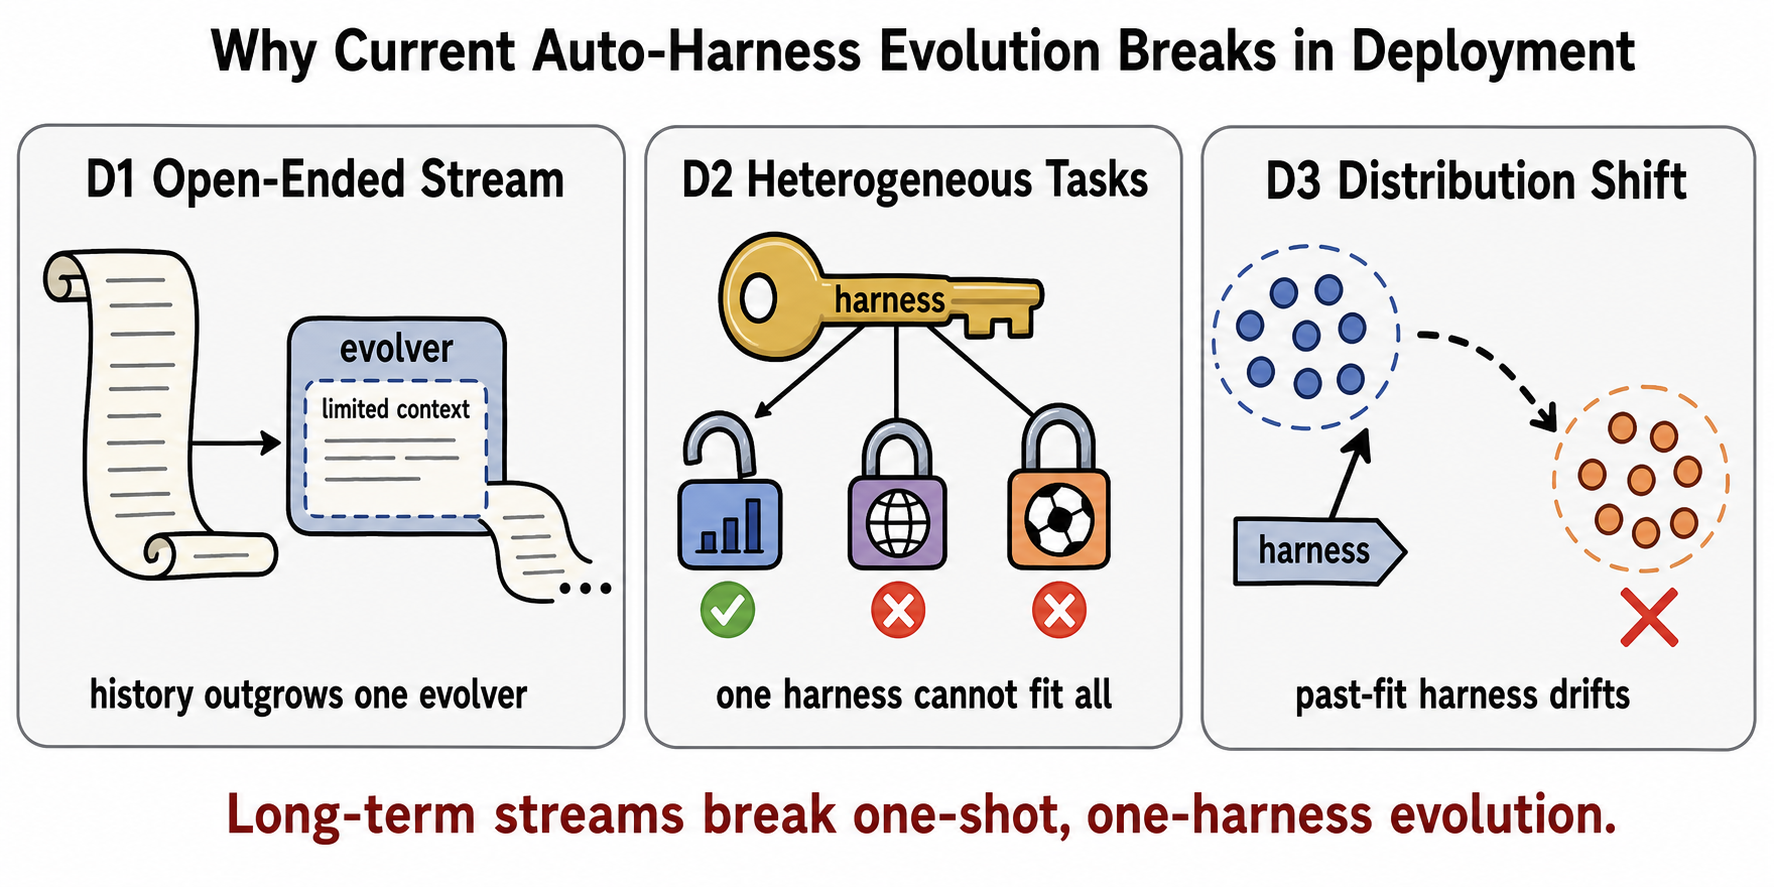
\includegraphics[width=\linewidth]{figures/generated/figure1_three_gap_metaphors.png}
\vspace{-0.5em}

\textbf{(a) Conceptual gaps.}

\vspace{0.4em}

\includegraphics[width=\linewidth]{figures/figure_c1_paper.pdf}
\vspace{-0.5em}

\textbf{(b) Empirical signature.}
\caption{\textbf{Deployment gaps in long-term auto-harness evolution.} (a) Long-running deployment exposes three gaps: history grows beyond a single evolver's effective capacity (D1), heterogeneous tasks require different harnesses (D2), and past-fit harnesses drift under distribution shift (D3). (b) On PolyBench, pass-rate lift is non-monotonic: a finite budget (30 cycles) peaks at $+10.6$ pp and beats unbounded evolution by $3.8$ pp.}
\label{fig:c1}
\end{figure}

{We address these three dimensions under a unified analytical framework and identify two axes of root gaps that prior auto-harness systems overlook. From the axis, we propose: (1) \emph{Continual auto-harness} (\S\ref{sec:method-multi}) replaces stateless one-shot evolution with a stateful multi-agent system with cross-cycle knowledge for better harness construction; (2) \emph{Runtime adaptation} (\S\ref{sec:method-nav}) adapts a task-relevant harness for each problem prior to solving, restoring per-task fit on a heterogeneous, drifting stream. Beyond the two axes, we further introduce a third axis: human-in-the-loop (HITL) for auxiliary steering of the harness to incorporate human insights and provisions that are absent from historical experience.} We summarize the contributions as follows:

\begin{compactenum}[(1)]
  \item {\textbf{Analytical framework for long-running agentic self-improvement.} We propose a regret decomposition that splits the gap to the optimal harness into a construction loss and an adaptation loss. The decomposition reveals two axes of root gaps in prior auto-harness systems and derives the two complementary operations: continual harness construction and solve-time adaptation, with a third human-in-the-loop channel for cases where accumulated experience is insufficient.}
  \item {\textbf{System-design novelties.} A stateful multi-agent evolver with cross-cycle knowledge realises continual auto-harness, replacing stateless one-shot evolution with cumulative construction; a strategy-tree navigator realises solve-time adaptation by selecting a task-relevant harness from a repertoire prior to solving; structurally triggered human-in-the-loop hooks handle regimes outside prior experience.}
  \item \textbf{Empirical validation on three real task streams.} We evaluate against A-Evolve, GEPA, and Meta-Harness on prediction-market, security-competition, and forecasting streams, with ablations isolating each operation's contribution.
\end{compactenum}






